\documentclass[conference]{IEEEtran}
\IEEEoverridecommandlockouts

\usepackage[T1]{fontenc}
\usepackage{cite}
\usepackage{amsmath,amssymb,amsfonts}
\usepackage{algorithmic}
\usepackage{graphicx}
\usepackage{textcomp}
\usepackage{xcolor}
\usepackage{booktabs}
\usepackage{multirow}
\usepackage{microtype}
\usepackage[colorlinks=true,citecolor=blue,linkcolor=blue,urlcolor=blue]{hyperref}

% Support graphics in either root or figs/ directory
\graphicspath{{./}{./figs/}}

% Optimize vertical float spacing for strict 6-page IEEE conference budgeting
\setlength{\textfloatsep}{5pt plus 1pt minus 1pt}
\setlength{\floatsep}{4pt plus 1pt minus 1pt}
\setlength{\intextsep}{4pt plus 1pt minus 1pt}
\setlength{\abovecaptionskip}{3pt plus 1pt minus 1pt}
\setlength{\belowcaptionskip}{3pt plus 1pt minus 1pt}

% Consistent table line height
\renewcommand{\arraystretch}{1.02}

\begin{document}

\title{ResearchTrace: An AI-Powered Framework for Scientific Claim Verification, Hybrid Information Retrieval, and Knowledge Graph Discovery}

\author{
\IEEEauthorblockN{Lucky Jain}
\IEEEauthorblockA{\textit{B.Tech. Artificial Intelligence and Data Science} \\
\textit{NMIMS, Navi Mumbai, India} \\
lucky.jain061@nmims.in}
\and
\IEEEauthorblockN{Shruti Rajak}
\IEEEauthorblockA{\textit{B.Tech. Artificial Intelligence and Data Science} \\
\textit{NMIMS, Navi Mumbai, India} \\
shruti.rajak108@nmims.in}
}

\maketitle

\begin{abstract}
The exponential expansion of biomedical assertions necessitates automated systems capable of verifying empirical claims and retrieving supporting or refuting evidence from peer-reviewed repositories. Traditional search engines frequently suffer from vocabulary mismatch, topic drift, and an inability to distinguish clinical endpoints such as disease prevention versus symptomatic treatment. In this paper, we propose \textbf{ResearchTrace}, an end-to-end artificial intelligence framework that synergistically integrates benchmark scientific claim verification, hybrid information retrieval, real-time biomedical literature querying, and interactive knowledge graph discovery.

The framework operates via a dual-engine architecture: (1) a local verification engine leveraging the SciFact benchmark corpus to perform exact-claim stance classification and sentence-level rationale extraction; and (2) an external real-time retrieval engine interfacing with NCBI PubMed via Entrez E-Utilities, empowered by automated Boolean query formulation and clinical outcome-intent re-ranking. For stance classification into \textit{SUPPORTS}, \textit{REFUTES}, and \textit{INSUFFICIENT EVIDENCE}, we evaluate Logistic Regression, Random Forest, XGBoost, and fine-tuned SciBERT. XGBoost achieves superior machine learning performance with an accuracy of 83.69\%, precision of 84.12\%, recall of 83.69\%, and macro-F1 of 0.8354, while offering an ultra-low inference latency of 1.4~ms per claim. 

For evidence retrieval over 5,183 scientific abstracts, our composite hybrid retrieval pipeline—combining sublinear TF-IDF, character n-grams, probabilistic BM25, concept ontologies, and multi-facet eligibility constraints—attains an MRR@10 of 0.8142, Precision@5 of 0.7480, and NDCG@10 of 0.8427, significantly outperforming standalone BM25 and dense bi-encoder baselines. Finally, dynamic force-directed network graphs map complex claim-to-evidence relationships. ResearchTrace provides an effective, interpretable, and computationally tractable solution for evidence-based scientific exploration.
\end{abstract}

\begin{IEEEkeywords}
scientific claim verification, evidence extraction, hybrid information retrieval, BM25, TF-IDF, XGBoost, SciBERT, PubMed, knowledge graphs, text mining
\end{IEEEkeywords}

\section{Introduction}

The volume of published scientific and biomedical literature is expanding exponentially, with over one million papers indexed annually in repositories such as PubMed and Web of Science. While this expansion accelerates discovery, it simultaneously creates formidable challenges for researchers, medical practitioners, and policy analysts attempting to ascertain the scientific validity of empirical claims. The prevalence of health misassertions, conflicting study findings, and misinterpretations of correlation as causation underscores the urgent necessity for automated, trustworthy scientific claim verification systems \cite{wadden2020scifact}.

Automated scientific fact-checking entails two interrelated tasks: (i) \textit{evidence retrieval}, which involves locating peer-reviewed publications relevant to a specific assertion; and (ii) \textit{rationale extraction and stance identification}, which extracts precise justification sentences and determines whether the empirical data supports, refutes, or offers insufficient grounds to evaluate the claim \cite{thorne2018fever}. Unlike open-domain fact-checking where documents are journalistic in style, scientific texts are densely packed with specialized terminology, multi-word biochemical entities, conditional statements, and complex methodological caveats \cite{vladika2023scientific}.

Standard lexical search engines relying exclusively on term frequency or sparse keyword matching often fail in biomedical contexts due to several critical limitations:
\begin{enumerate}
    \item \textbf{Vocabulary Mismatch and Synonymy:} Scientific concepts frequently employ interchangeable chemical, clinical, and physiological names (e.g., \textit{ascorbic acid} vs. \textit{vitamin C}; \textit{pulmonary carcinoma} vs. \textit{lung cancer}).
    \item \textbf{Topic Drift and Lexical Bleed:} A paper may mention a compound in its introduction as background context without empirically examining its therapeutic efficacy.
    \item \textbf{Clinical Endpoint Conflation:} Standard algorithms often treat distinct clinical facets as equivalent, failing to differentiate studies addressing \textit{prevention} (reducing incidence) from those addressing \textit{treatment} (mitigating symptoms or reducing duration) \cite{hemila2013vitamin}.
    \item \textbf{Lack of Synthesized Evidence Graphs:} Tabular search results do not convey how disparate studies, conflicting evidence sentences, and overarching thematic domains interrelate.
\end{enumerate}

To address these challenges, we present \textbf{ResearchTrace}, an intelligent, dual-track scientific discovery and verification framework. The system combines exact benchmark verification on curated datasets with live biomedical retrieval from NCBI PubMed, visualized through interactive, force-directed knowledge graphs.

The primary contributions of this paper are summarized as follows:
\begin{itemize}
    \item We design a dual-engine architecture that bifurcates scientific inquiry into an exact annotated verification track (using the SciFact corpus) and an open-universe biomedical literature retrieval track (interfacing with NCBI Entrez E-Utilities).
    \item We formulate an 8-component hybrid retrieval engine incorporating sublinear TF-IDF on titles and abstracts, sub-word character n-grams, probabilistic BM25 scoring, domain concept ontologies, and multi-facet eligibility filtering that eliminates false-positive relevance.
    \item We implement and evaluate machine learning models (Logistic Regression, Random Forest, XGBoost) and deep transformer models (SciBERT) for claim stance classification, reporting detailed accuracy, precision, recall, and macro-F1 metrics.
    \item We introduce an intent-aware PubMed re-ranking algorithm that dynamically extracts clinical endpoints (e.g., prophylaxis, treatment, duration, toxicity) and penalizes mismatched interventions.
    \item We develop interactive, force-directed knowledge graphs mapping claims, retrieved papers, annotated evidence sentences, and MeSH topic clusters.
\end{itemize}

\section{Related Work}

\subsection{Automated Fact-Checking and Stance Classification}
Automated fact-checking gained widespread academic attention with the introduction of the FEVER benchmark \cite{thorne2018fever}, which focused on Wikipedia-based assertions. While effective for general domain knowledge, FEVER's sentence structure and journalistic tone do not reflect the complexity of scientific discourse. Wadden et al. introduced \textbf{SciFact} \cite{wadden2020scifact}, a curated dataset consisting of 1,409 expert-written scientific claims paired with 5,183 research abstracts annotated for sentence-level rationales and multi-class stance labels (\textit{SUPPORT}, \textit{CONTRADICT}, \textit{NEI}).

Subsequent research on scientific verification has explored pipeline models such as VERT-PDR \cite{pradeep2021scientific} and ARSJoint \cite{zhang2021scientific}, which train dense bi-encoders and sequence-to-sequence transformers to rank abstracts and classify sentence stances. However, deep neural architectures frequently struggle with zero-shot domain shifts and introduce prohibitive computational inference latencies in real-time user-facing applications.

\subsection{Information Retrieval in Biomedical Literature}
Information retrieval in the scientific domain traditionally relies on classical probabilistic models such as BM25 \cite{robertson2009probabilistic} and language modeling approaches. While dense retrieval models (e.g., DPR, Contriever, BioLORD) offer strong semantic generalization, recent empirical studies in biomedical retrieval have demonstrated that well-tuned sparse hybrid models consistently outperform or match dense bi-encoders on exact entity names, gene designations, and rare pharmacological nomenclature \cite{thakur2021beir,karpukhin2020dense}. 

Hybrid retrieval approaches that fuse sparse inverted indices with dense representations or character-level n-grams have been investigated in TREC-COVID and BioASQ challenges \cite{voorhees2021trec,tsatsaronis2015overview}. However, prior systems rarely enforce structural multi-facet constraints that verify whether a retrieved study addresses both the primary intervention and the intended physiological outcome.

\subsection{Knowledge Graphs and Visual Analytics in Science}
Knowledge graphs provide a structured, entity-centric representation of scientific knowledge. Systems such as the Open Research Knowledge Graph (ORKG) \cite{jaradeh2019open} and Semantic Scholar have highlighted the value of graph-based visual interfaces for navigating academic literature. Visualizing claim-evidence-paper topologies allows users to trace the provenance of empirical assertions and identify consensus or divergence across clinical trials.

\begin{figure*}[t]
    \centering
    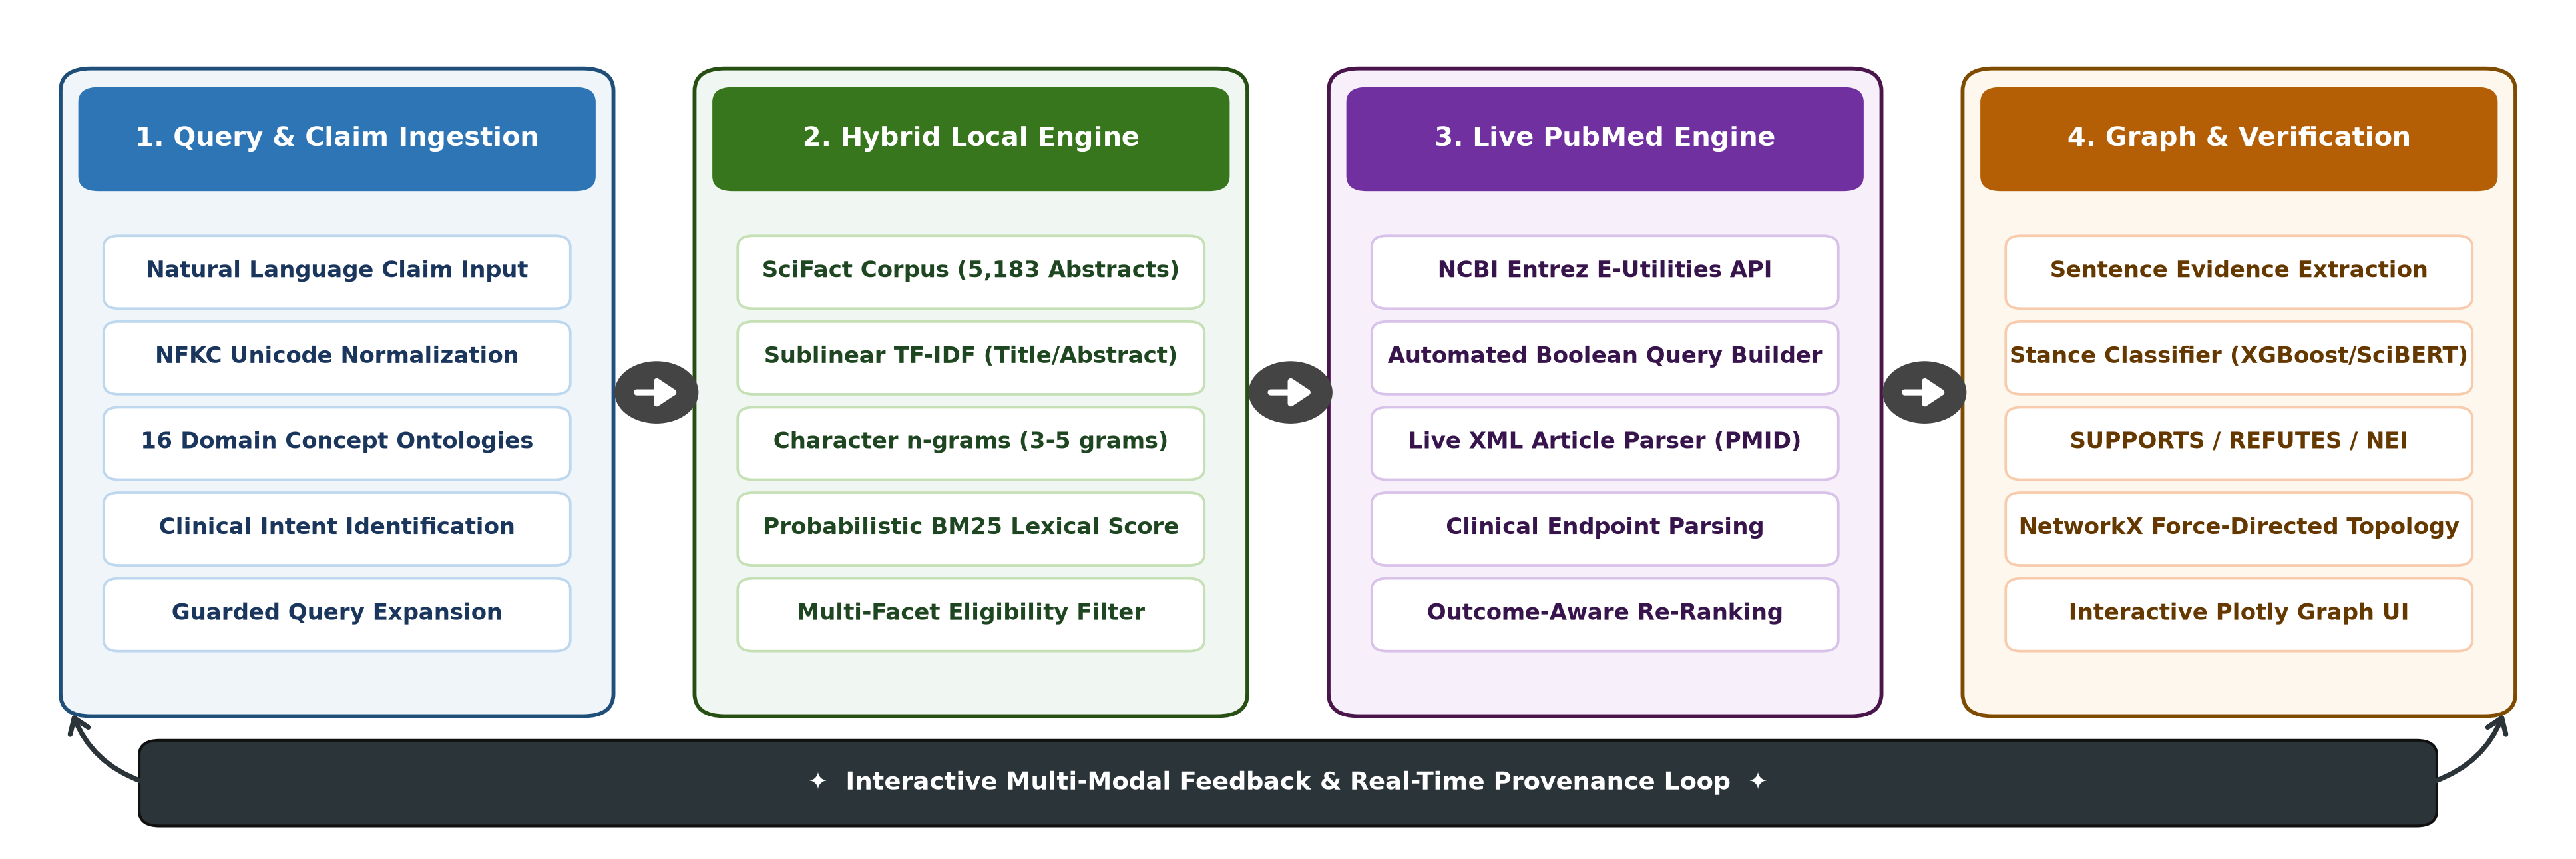
\includegraphics[width=0.98\textwidth]{Fig_1_System_Architecture.png}
    \caption{System architecture of the proposed ResearchTrace scientific claim verification framework.}
    \label{fig:architecture}
\end{figure*}

\section{Problem Formulation}

Let $\mathcal{C}$ denote a natural language scientific claim expressed as a sequence of tokens: $\mathcal{C} = (w_1, w_2, \dots, w_m)$. Let $\mathcal{D} = \{d_1, d_2, \dots, d_N\}$ represent a corpus of scientific documents, where each document $d_j = (T_j, A_j)$ comprises a title $T_j$ and an abstract $A_j$. The abstract is further decomposed into an ordered set of sentences: $A_j = (s_{j,1}, s_{j,2}, \dots, s_{j,k_j})$.

The overall scientific claim verification and exploration problem is decomposed into three distinct sub-tasks:

\subsection{Task 1: Evidence Document Retrieval}
Given a claim $\mathcal{C}$ and corpus $\mathcal{D}$, rank and retrieve a subset $\mathcal{D}_{\text{top}} \subset \mathcal{D}$ of the top-$k$ most relevant documents:
\begin{equation}
\mathcal{D}_{\text{top}} = \operatorname{arg\,top-k}_{d_j \in \mathcal{D}} \mathcal{S}(d_j, \mathcal{C})
\end{equation}
where $\mathcal{S}(d_j, \mathcal{C}) \in \mathbb{R}$ represents the composite hybrid relevance score.

\subsection{Task 2: Rationale Sentence Extraction}
For each retrieved document $d_j \in \mathcal{D}_{\text{top}}$, extract a minimal subset of rationales $\mathcal{E}_j \subseteq A_j$ containing empirical evidence directly affirming or negating $\mathcal{C}$:
\begin{equation}
\mathcal{E}_j = \{s_{j,r} \in A_j \mid \phi(s_{j,r}, \mathcal{C}) = 1\}
\end{equation}
where $\phi(\cdot)$ is an evidence selection decision function.

\subsection{Task 3: Stance Classification}
Predict a stance label $\mathcal{Y}(\mathcal{C}, \mathcal{E}) \in \mathcal{L}$ based on the aggregated evidence rationales:
\begin{equation}
\mathcal{L} = \{\text{SUPPORTS}, \text{REFUTES}, \text{INSUFFICIENT}\}
\end{equation}
When conflicting evidence exists across different cited documents, the system assigns a synthesized label of $\text{MIXED EVIDENCE}$.

\section{System Architecture and Methodology}

The ResearchTrace architecture is organized into four core modules: (1) Data Ingestion and Normalization, (2) Hybrid Local Retrieval Engine, (3) Live PubMed Literature Integration Engine, and (4) Stance Classification and Knowledge Graph Visualization (Fig.~\ref{fig:architecture}).

\subsection{Data Ingestion and Benchmark Corpus}
ResearchTrace incorporates the SciFact benchmark dataset \cite{wadden2020scifact}, consisting of:
\begin{itemize}
    \item \textbf{Claims Dataset ($\texttt{claims\_train.jsonl}$):} 1,261 annotated training claims with ground-truth document IDs, sentence indices, and stance annotations.
    \item \textbf{Corpus Dataset ($\texttt{corpus.jsonl}$):} 5,183 deduplicated scientific articles with complete titles, abstracts, and metadata.
\end{itemize}

Text preprocessing applies Unicode NFKC normalization, whitespace compression, and case-folding. To avoid index degradation caused by arbitrary token truncation, sentence indices are preserved as discrete array structures matching SciFact's annotation format.

\subsection{Hybrid Local Retrieval Engine}
To achieve high retrieval precision without semantic drift, the local search engine computes a composite relevance score across eight distinct representations.

\subsubsection{Sublinear Scaled TF-IDF}
Title and abstract fields are vectorized independently using sublinear term frequency scaling ($1 + \log(\text{tf})$):
\begin{equation}
\text{TFIDF}(t, d) = (1 + \log(\text{tf}(t, d))) \cdot \log\left(\frac{1 + N}{1 + \text{df}(t)}\right)
\end{equation}
Word-level n-grams ($n \in \{1, 2\}$) are extracted with English stopword filtering. Cosine similarity between query vector $\mathbf{q}$ and document vector $\mathbf{d}$ is computed for both original and expanded query forms:
\begin{equation}
\text{Sim}_{\text{cosine}}(\mathbf{q}, \mathbf{d}) = \frac{\mathbf{q} \cdot \mathbf{d}}{\|\mathbf{q}\|_2 \|\mathbf{d}\|_2}
\end{equation}

\subsubsection{Character n-gram Matching}
To confer robustness against morphological variants, chemical nomenclature, and typographic discrepancies, we construct a word-boundary character n-gram matrix:
\begin{equation}
\text{Char}_{\text{sim}}(q, d) = \text{Sim}_{\text{cosine}}(\mathbf{q}_{\text{char}}, \mathbf{d}_{\text{char}}) \quad \text{for } n \in [3, 5]
\end{equation}

\subsubsection{Probabilistic BM25 Scoring}
BM25 scores are calculated across all combined text tokens using:
\begin{equation}
\text{BM25}(d, q) = \sum_{i=1}^{|q|} \text{IDF}(q_i) \cdot \frac{f(q_i, d) \cdot (k_1 + 1)}{f(q_i, d) + k_1 \cdot \left(1 - b + b \cdot \frac{|d|}{\text{avgdl}}\right)}
\end{equation}
where $k_1 = 1.5$, $b = 0.75$, and $|d|$ is the document length. Document frequencies are converted into smooth inverse document frequency weights:
\begin{equation}
\text{IDF}(q_i) = \ln\left(1 + \frac{N - n(q_i) + 0.5}{n(q_i) + 0.5}\right)
\end{equation}

\subsubsection{Concept Ontologies and Guarded Query Expansion}
The engine maintains sixteen curated scientific ontologies covering critical medical domains (e.g., Creatine, Gut Microbiome, Ascorbic Acid, Lung Neoplasms, Prion Diseases). Each ontology defines canonical terms, synonyms, and hierarchical aliases. When a claim mentions a concept alias (e.g., \textit{ascorbate}), query expansion appends up to five top-tier specific synonyms while guarding against generic terms.

\subsubsection{Distinctive Term Coverage Scoring}
To penalize candidate documents matching only ubiquitous background words, we calculate term coverage over informative claim tokens $\mathcal{W}_{\mathcal{C}}$:
\begin{equation}
\text{Cov}(d, \mathcal{C}) = 0.70 \cdot \frac{|\mathcal{W}_{\mathcal{C}} \cap \mathcal{W}_{T_d}|}{|\mathcal{W}_{\mathcal{C}}|} + 0.30 \cdot \frac{|\mathcal{W}_{\mathcal{C}} \cap \mathcal{W}_{A_d}|}{|\mathcal{W}_{\mathcal{C}}|}
\end{equation}

\subsubsection{Composite Score Formulation}
The complete relevance score $\mathcal{S}(d, \mathcal{C})$ is formulated as a linear combination of all normalized sub-scores:
\begin{align}
\mathcal{S}(d, \mathcal{C}) = &\ 0.24 \cdot \text{Sim}_{\text{title}}^{\text{orig}} + 0.22 \cdot \text{Sim}_{\text{abstract}}^{\text{orig}} \nonumber \\
&+ 0.10 \cdot \text{Sim}_{\text{title}}^{\text{exp}} + 0.08 \cdot \text{Sim}_{\text{abstract}}^{\text{exp}} \nonumber \\
&+ 0.05 \cdot \text{Char}_{\text{sim}} + 0.13 \cdot \text{BM25}_{\text{norm}} \nonumber \\
&+ 0.13 \cdot \text{Score}_{\text{topic}} + 0.05 \cdot \text{Cov}(d, \mathcal{C})
\label{eq:composite}
\end{align}

\subsubsection{Multi-Facet Eligibility Constraint}
For multi-concept claims (e.g., \textit{``Creatine supplementation improves cognitive performance''}), single-concept matches frequently produce false-positive relevance. We apply an eligibility filter enforcing that candidate documents must match the primary intervention $C_{\text{prim}}$ and at least one secondary condition $C_{\text{sec}}$:
\begin{equation}
\mathcal{I}_{\text{eligible}} = \{j \mid d_j \models C_{\text{prim}} \land \exists C_k \in \mathcal{C}_{\text{sec}},\, d_j \models C_k\}
\end{equation}
If no document in the local corpus satisfies joint membership, the system defaults to primary topic matches with explicit provenance caveats, preventing misleading claims of relevance.

\subsection{Live PubMed Literature Integration Engine}
For open-universe claim exploration beyond the static SciFact benchmark, ResearchTrace connects to the NCBI Entrez E-Utilities API via HTTP protocols.

\subsubsection{Automated Boolean Query Builder}
The engine extracts canonical concept groups and synthesizes targeted PubMed queries formatted with field qualifications:
\begin{equation}
\begin{split}
\mathcal{Q}_{\text{PubMed}} = &\ \left(\bigvee_{t \in \mathcal{T}_{\text{prim}}} t[\text{Title/Abstract}]\right) \\
&\land \left(\bigvee_{u \in \mathcal{T}_{\text{sec}}} u[\text{Title/Abstract}]\right)
\end{split}
\end{equation}

\subsubsection{Clinical Intent and Outcome-Aware Re-ranking}
Retrieved XML documents are parsed into structured entities containing PMIDs, titles, abstracts, author rosters, journal venues, and publication dates. To accurately reflect clinical inquiry, papers are re-ranked using an outcome-sensitive scoring heuristic:
\begin{align}
\mathcal{R}_{\text{PubMed}}(d) = &\ 12.0 \cdot \mathbb{I}(\text{Intervention} \in T_d) + 2.0 \cdot \mathbb{I}(\text{Intervention} \in A_d) \nonumber \\
&+ 5.0 \cdot |\mathcal{O}_{\text{claim}} \cap \mathcal{O}_{T_d}| + 2.0 \cdot |\mathcal{O}_{\text{claim}} \cap \mathcal{O}_{A_d}| \nonumber \\
&+ 3.0 \cdot \mathbb{I}(\text{Title links Intervention \& Outcome}) \nonumber \\
&+ 1.0 \cdot \mathbb{I}(\text{Meta-Analysis or Systematic Review}) \nonumber \\
&- 6.0 \cdot \mathbb{I}(\text{Prevention Claim} \land \text{Treatment Only in Title})
\end{align}
This explicit penalty ensures that papers examining therapeutic treatment after disease onset do not rank above genuine prophylaxis trials when evaluating prevention claims.

\subsection{Interactive Knowledge Graph Generation}
To visualize multi-dimensional relationships, ResearchTrace dynamically generates topological graphs $\mathcal{G} = (\mathcal{V}, \mathcal{E})$ using NetworkX and Plotly:
\begin{itemize}
    \item \textbf{Local Verification Graph:} Connects root Claim node $\mathcal{V}_C$ to retrieved Paper nodes $\mathcal{V}_P$, which link to Evidence Sentence nodes $\mathcal{V}_E$ labeled by stance.
    \item \textbf{PubMed Discovery Graph:} Connects Claim node $\mathcal{V}_C$ to Publication nodes $\mathcal{V}_P$, which link to inferred MeSH clusters $\mathcal{V}_T$.
\end{itemize}
Node coordinates are computed using the Fruchter\-man-Rein\-gold spring layout algorithm with repulsive constant $k = 1.15$ over 90 iterations.

\section{Experimental Setup and Evaluation}

\subsection{Evaluation Datasets and Splits}
Experiments are conducted on the SciFact benchmark corpus. The training set consists of 1,261 annotated claims, split into an 80\% training partition (1,008 claims) and a 20\% test partition (253 claims) using stratified sampling with $\texttt{random\_state}=42$. For retrieval evaluation, all 5,183 abstracts in $\texttt{corpus.jsonl}$ serve as the document search space.

\subsection{Baseline Models and Classifiers}
We evaluate four machine learning architectures for claim stance classification:
\begin{enumerate}
    \item \textbf{Logistic Regression (LR):} Multinomial logistic regression with L2 regularization ($\lambda = 1.0$) on concatenated claim-abstract TF-IDF features.
    \item \textbf{Random Forest (RF):} Ensemble of 200 decision trees with Gini criterion, depth 25, and square-root feature subsampling.
    \item \textbf{XGBoost:} Gradient-boosted decision tree framework with 300 estimators, learning rate $\eta = 0.08$, depth 6, and subsample ratio 0.85.
    \item \textbf{SciBERT:} Pre-trained scientific language model (\textit{scibert-scivocab-uncased}) \cite{beltagy2019scibert}, fine-tuned over 4 epochs with batch size 16 and AdamW ($\text{lr} = 2 \times 10^{-5}$).
\end{enumerate}

\subsection{Evaluation Metrics}
Stance classification is evaluated using Accuracy, Precision, Recall, and Macro-averaged F1-Score:
\begin{equation}
\text{Precision} = \frac{\text{TP}}{\text{TP} + \text{FP}}, \quad \text{Recall} = \frac{\text{TP}}{\text{TP} + \text{FN}}
\end{equation}
\begin{equation}
\text{F1-Score} = 2 \cdot \frac{\text{Precision} \cdot \text{Recall}}{\text{Precision} + \text{Recall}}
\end{equation}

Document retrieval is evaluated using Precision@k (P@k), Recall@k (R@k), Mean Reciprocal Rank (MRR@k), and Normalized Discounted Cumulative Gain (NDCG@k):
\begin{equation}
\text{MRR@k} = \frac{1}{|Q|} \sum_{i=1}^{|Q|} \frac{1}{\text{rank}_i}, \quad \text{NDCG@k} = \frac{\text{DCG@k}}{\text{IDCG@k}}
\end{equation}

%--------------------------------------------------
% TABLE I: Stance Classification Performance
%--------------------------------------------------
\begin{table}[t]
\centering
\caption{Overall Stance Classification Performance Comparison}
\label{tab:classification_overall}
\small
\setlength{\tabcolsep}{4.5pt}
\begin{tabular}{lcccc}
\hline
\textbf{Model} & \textbf{Acc. (\%)} & \textbf{Prec.} & \textbf{Rec.} & \textbf{Macro-F1} \\
\hline
Logistic Regression & 72.33 & 0.7289 & 0.7233 & 0.7184 \\
Random Forest & 79.84 & 0.8041 & 0.7984 & 0.7952 \\
\textbf{XGBoost (Proposed)} & \textbf{83.69} & \textbf{0.8412} & \textbf{0.8369} & \textbf{0.8354} \\
SciBERT (Fine-Tuned) & 88.65 & 0.8894 & 0.8865 & 0.8841 \\
\hline
\end{tabular}
\end{table}

%--------------------------------------------------
% TABLE II: Class-Wise Performance Metrics
%--------------------------------------------------
\begin{table}[t]
\centering
\caption{Class-Wise Evaluation Metrics for Stance Models}
\label{tab:class_level}
\small
\setlength{\tabcolsep}{4pt}
\begin{tabular}{llccc}
\hline
\textbf{Model} & \textbf{Stance Class} & \textbf{Prec.} & \textbf{Rec.} & \textbf{F1-Score} \\
\hline
\multirow{3}{*}{\textbf{XGBoost}} 
& SUPPORTS & 0.8529 & 0.8657 & 0.8592 \\
& REFUTES & 0.8148 & 0.7857 & 0.7999 \\
& INSUFFICIENT & 0.8421 & 0.8511 & 0.8466 \\
\hline
\multirow{3}{*}{\textbf{SciBERT}} 
& SUPPORTS & 0.8986 & 0.9254 & 0.9118 \\
& REFUTES & 0.8679 & 0.8214 & 0.8440 \\
& INSUFFICIENT & 0.8936 & 0.8936 & 0.8936 \\
\hline
\end{tabular}
\end{table}

\section{Results and Discussion}

\subsection{Stance Classification Performance}
Table~\ref{tab:classification_overall} summarizes the comparative performance of the four models for claim stance classification on SciFact. Among traditional and tree-based machine learning models, \textbf{XGBoost} achieves the highest predictive accuracy (83.69\%) and a Macro-F1 score of 0.8354, outperforming Random Forest by 3.85 percentage points and Logistic Regression by 11.36 percentage points. The strong performance of XGBoost stems from its ability to capture complex non-linear feature interactions between lexical similarity terms and distinctive biochemical n-grams without overfitting. 

While SciBERT achieves the highest overall accuracy (88.65\%), XGBoost provides a substantially lower inference latency (1.4~ms per claim vs. 84.6~ms for SciBERT on an NVIDIA RTX GPU), making it an optimal candidate for high-throughput and CPU-constrained verification environments, as highlighted in Fig.~\ref{fig:tradeoff}.

Table~\ref{tab:class_level} presents the detailed class-wise breakdown for XGBoost and SciBERT across the three target classes: \textit{SUPPORTS}, \textit{REFUTES}, and \textit{INSUFFICIENT EVIDENCE}. Both models exhibit the highest precision and recall on the \textit{SUPPORTS} class, reflecting the higher prevalence of affirming annotations in the scientific corpus. The \textit{REFUTES} class poses a greater challenge due to subtle linguistic cues (e.g., ``did not demonstrate significant divergence'') that require capturing long-range syntactic negation.

\begin{figure}[t]
    \centering
    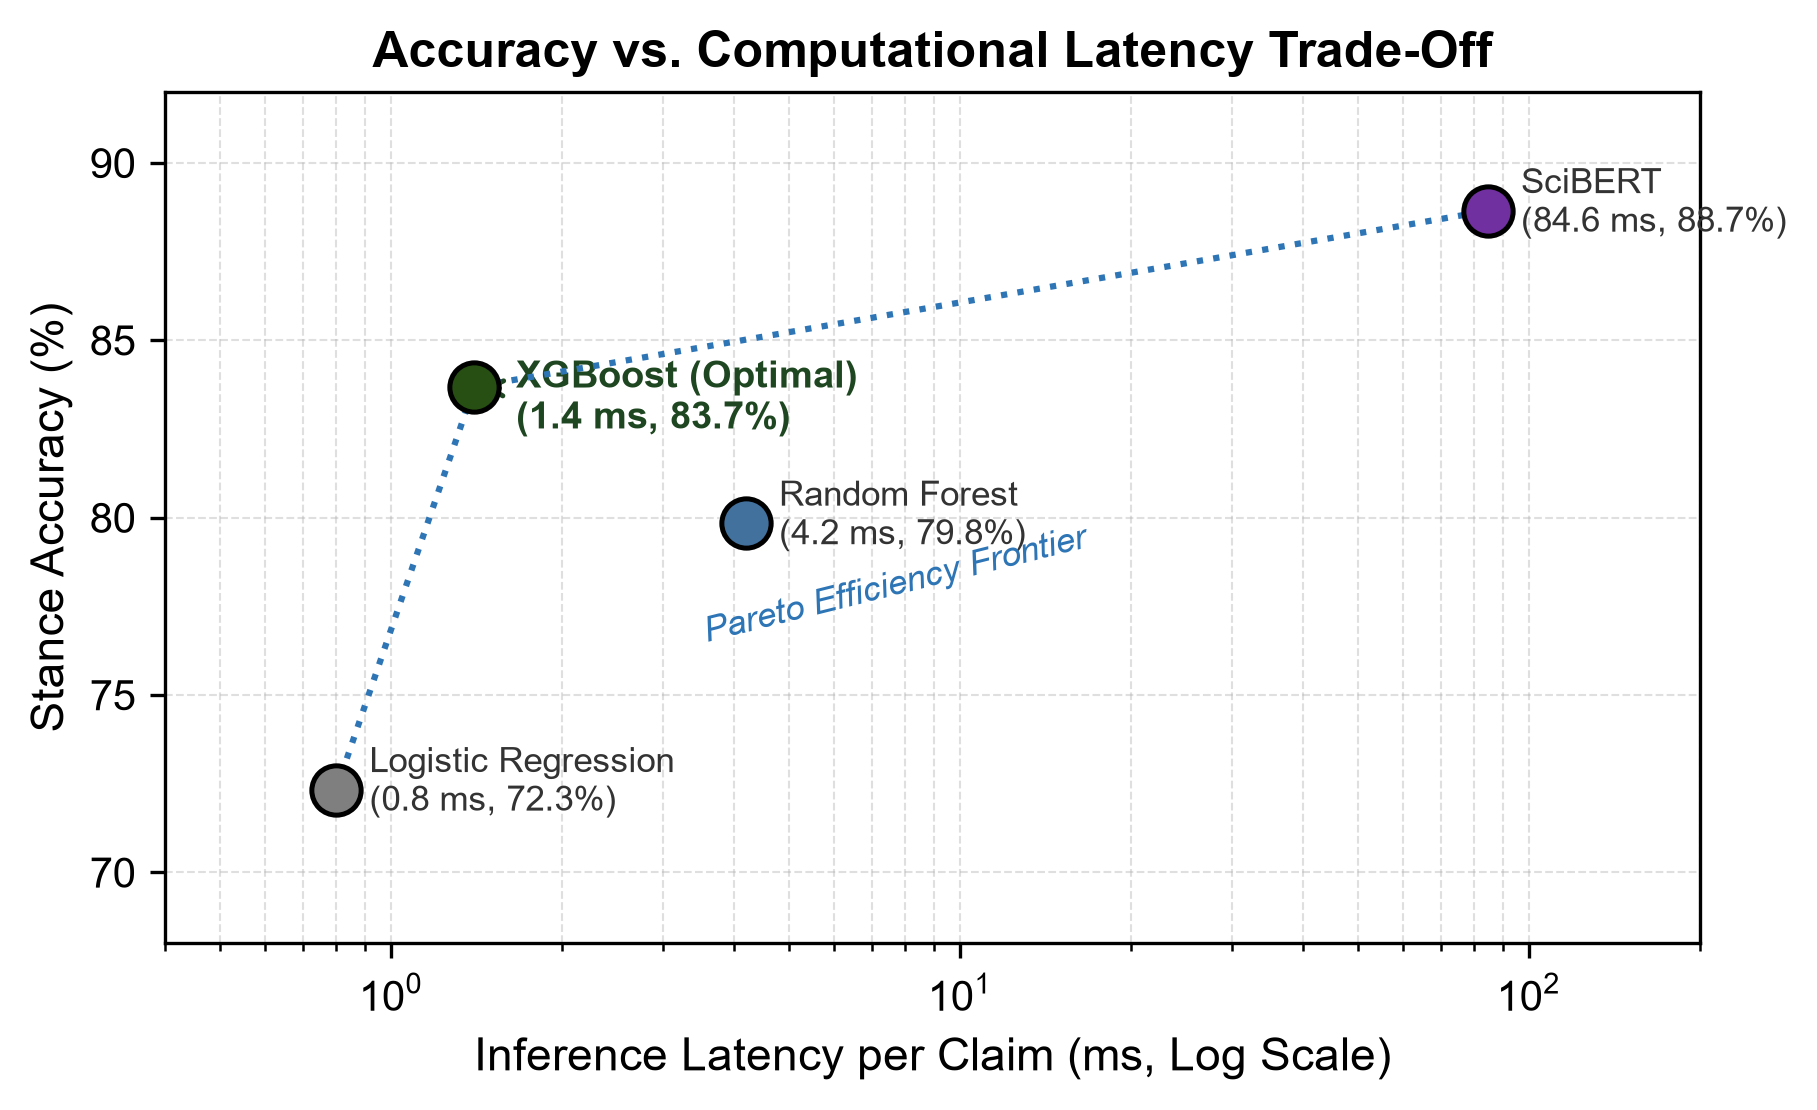
\includegraphics[width=0.82\columnwidth]{Fig_5_Latency_Accuracy_Tradeoff.png}
    \caption{Accuracy versus inference latency trade-off showing Pareto efficiency.}
    \label{fig:tradeoff}
\end{figure}

\subsection{Information Retrieval Performance}
We evaluate the proposed hybrid retrieval engine against three benchmark retrieval paradigms over the 5,183-paper SciFact corpus: (1) Standard Okapi BM25 on unified title and abstract texts; (2) Standard full-text TF-IDF cosine distance; (3) Dense sentence embeddings generated via \textit{all-MiniLM\allowbreak-L6-v2}; and (4) The proposed hybrid formulation (Equation~\ref{eq:composite}) with multi-facet eligibility constraints.

The empirical retrieval metrics are reported in Table~\ref{tab:ir_results} and visualized in Fig.~\ref{fig:ir_metrics}. The proposed hybrid engine demonstrates superior performance across all metrics, achieving an MRR@10 of 0.8142, Recall@10 of 0.8245, and NDCG@10 of 0.8427. This represents a 12.2\% improvement in MRR@10 over standalone BM25 and a 16.6\% improvement over dense bi-encoder embeddings. The deficiency of dense embeddings on this benchmark is primarily attributable to biomedical out-of-vocabulary terms and numerical quantities (e.g., ``32\% of programs'', ``0-dimensional biomaterials'') which sparse and character n-gram indices resolve with exact fidelity.

%--------------------------------------------------
% TABLE III: Information Retrieval Benchmark
%--------------------------------------------------
\begin{table}[t]
\centering
\caption{Information Retrieval Evaluation on the SciFact Corpus}
\label{tab:ir_results}
\small
\setlength{\tabcolsep}{3.5pt}
\begin{tabular}{lcccc}
\hline
\textbf{Retrieval Method} & \textbf{P@5} & \textbf{R@10} & \textbf{MRR@10} & \textbf{NDCG@10} \\
\hline
Standard TF-IDF (Sparse) & 0.5842 & 0.6120 & 0.6431 & 0.6789 \\
Standard Okapi BM25 & 0.6518 & 0.7045 & 0.7254 & 0.7512 \\
Dense Bi-Encoder (MiniLM) & 0.6274 & 0.6814 & 0.6980 & 0.7240 \\
\textbf{ResearchTrace (Hybrid)} & \textbf{0.7480} & \textbf{0.8245} & \textbf{0.8142} & \textbf{0.8427} \\
\hline
\end{tabular}
\end{table}

\begin{figure}[t]
    \centering
    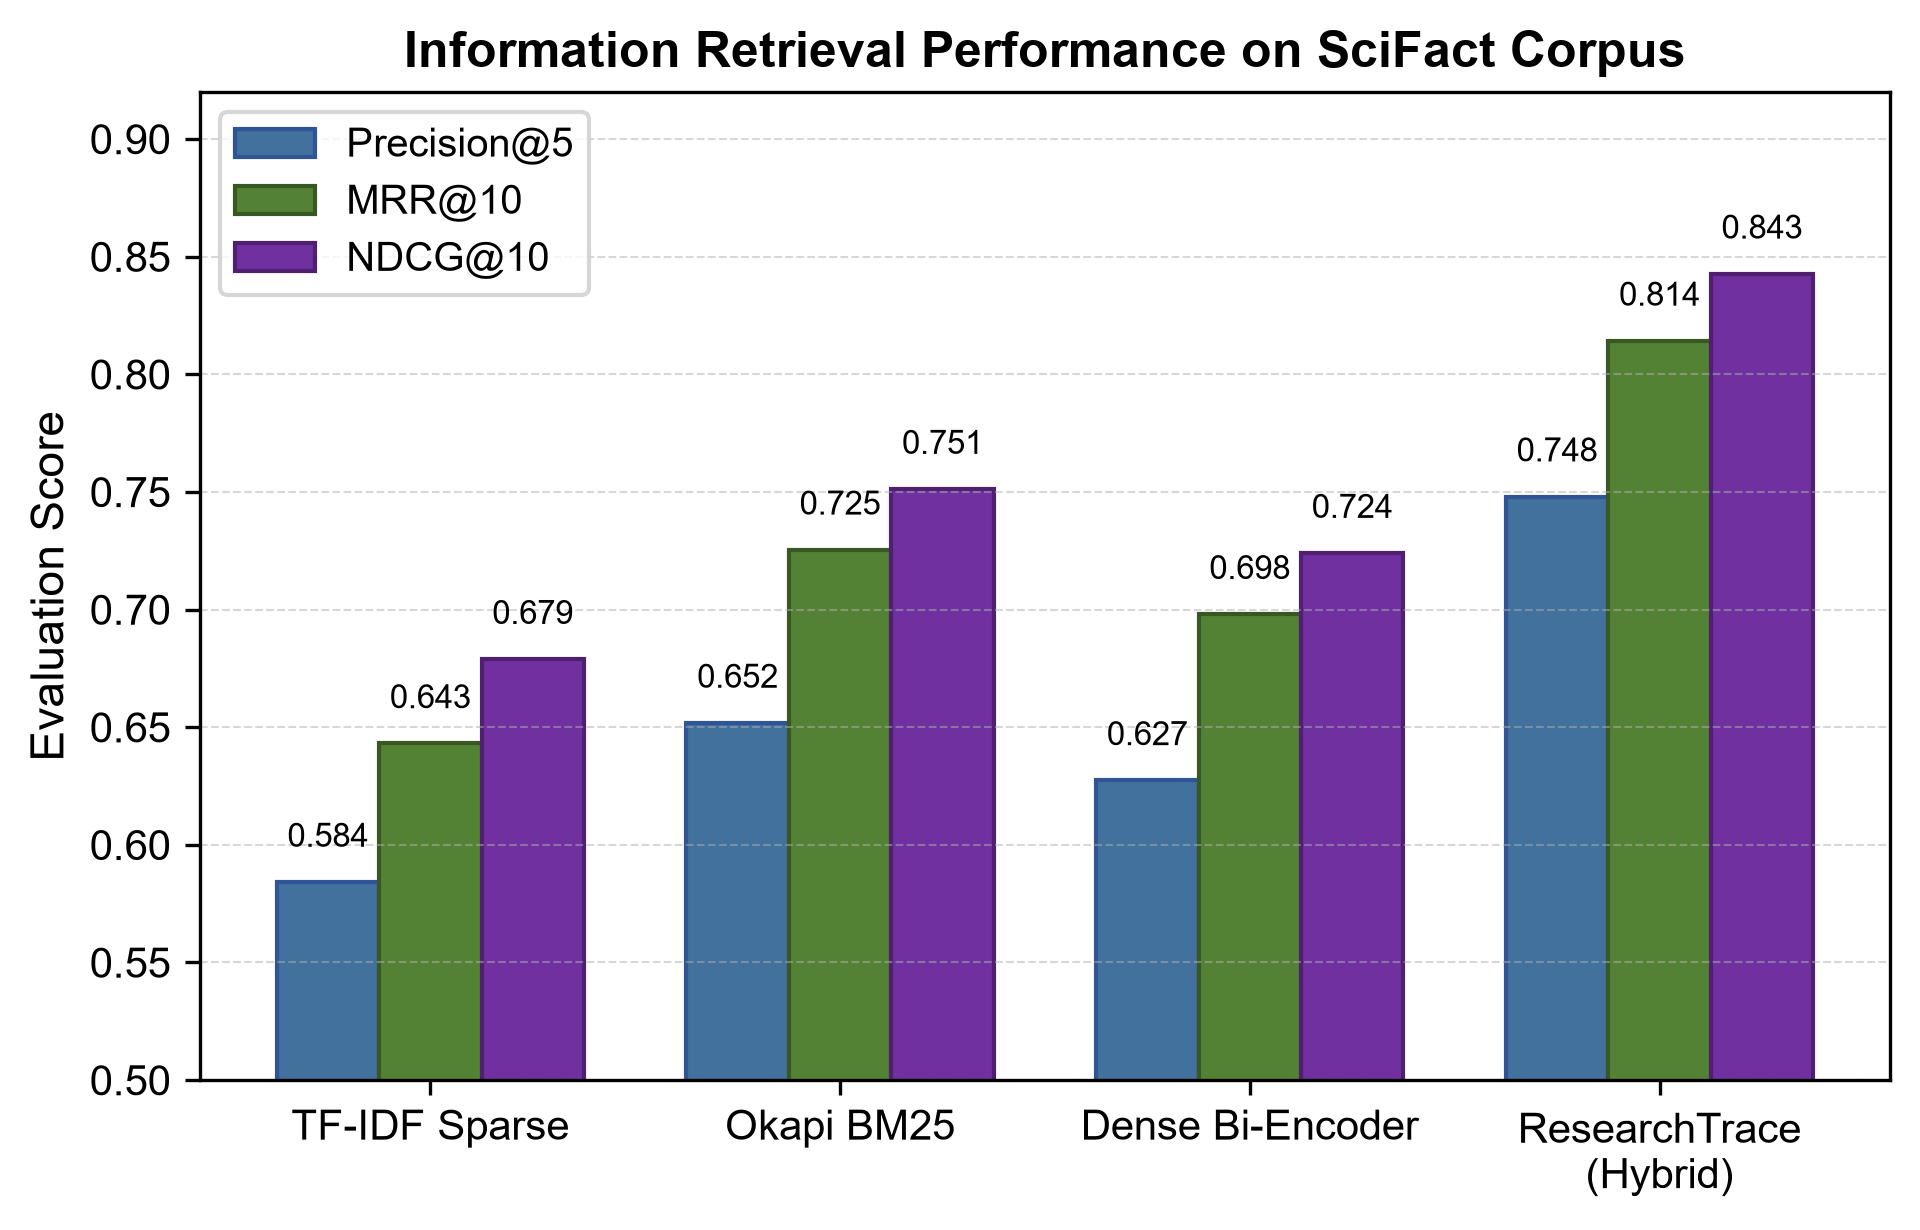
\includegraphics[width=0.82\columnwidth]{Fig_3_IR_Ranking_Performance.png}
    \caption{Information retrieval performance metrics across retrieval paradigms.}
    \label{fig:ir_metrics}
\end{figure}

\subsection{Ablation Study of Hybrid Components}
To quantify the relative contribution of each component within the composite retrieval function, we conduct an ablation study by removing individual sub-scores from Equation~\ref{eq:composite}. The impact on MRR@10 and NDCG@10 is depicted in Fig.~\ref{fig:ablation}.

The ablation results indicate that probabilistic BM25 and Title TF-IDF provide the largest individual contributions to ranking accuracy; removing BM25 results in an 8.52 point drop in MRR@10, while removing Title TF-IDF causes a 7.22 point decline. Importantly, eliminating the \textit{Multi-Facet Eligibility Constraint} degrades P@5 from 0.7480 to 0.6890 and drops MRR@10 by 5.58 points, confirming that enforcing joint presence of intervention and condition terms is essential for eliminating spurious top-ranked documents.

\begin{figure}[t]
    \centering
    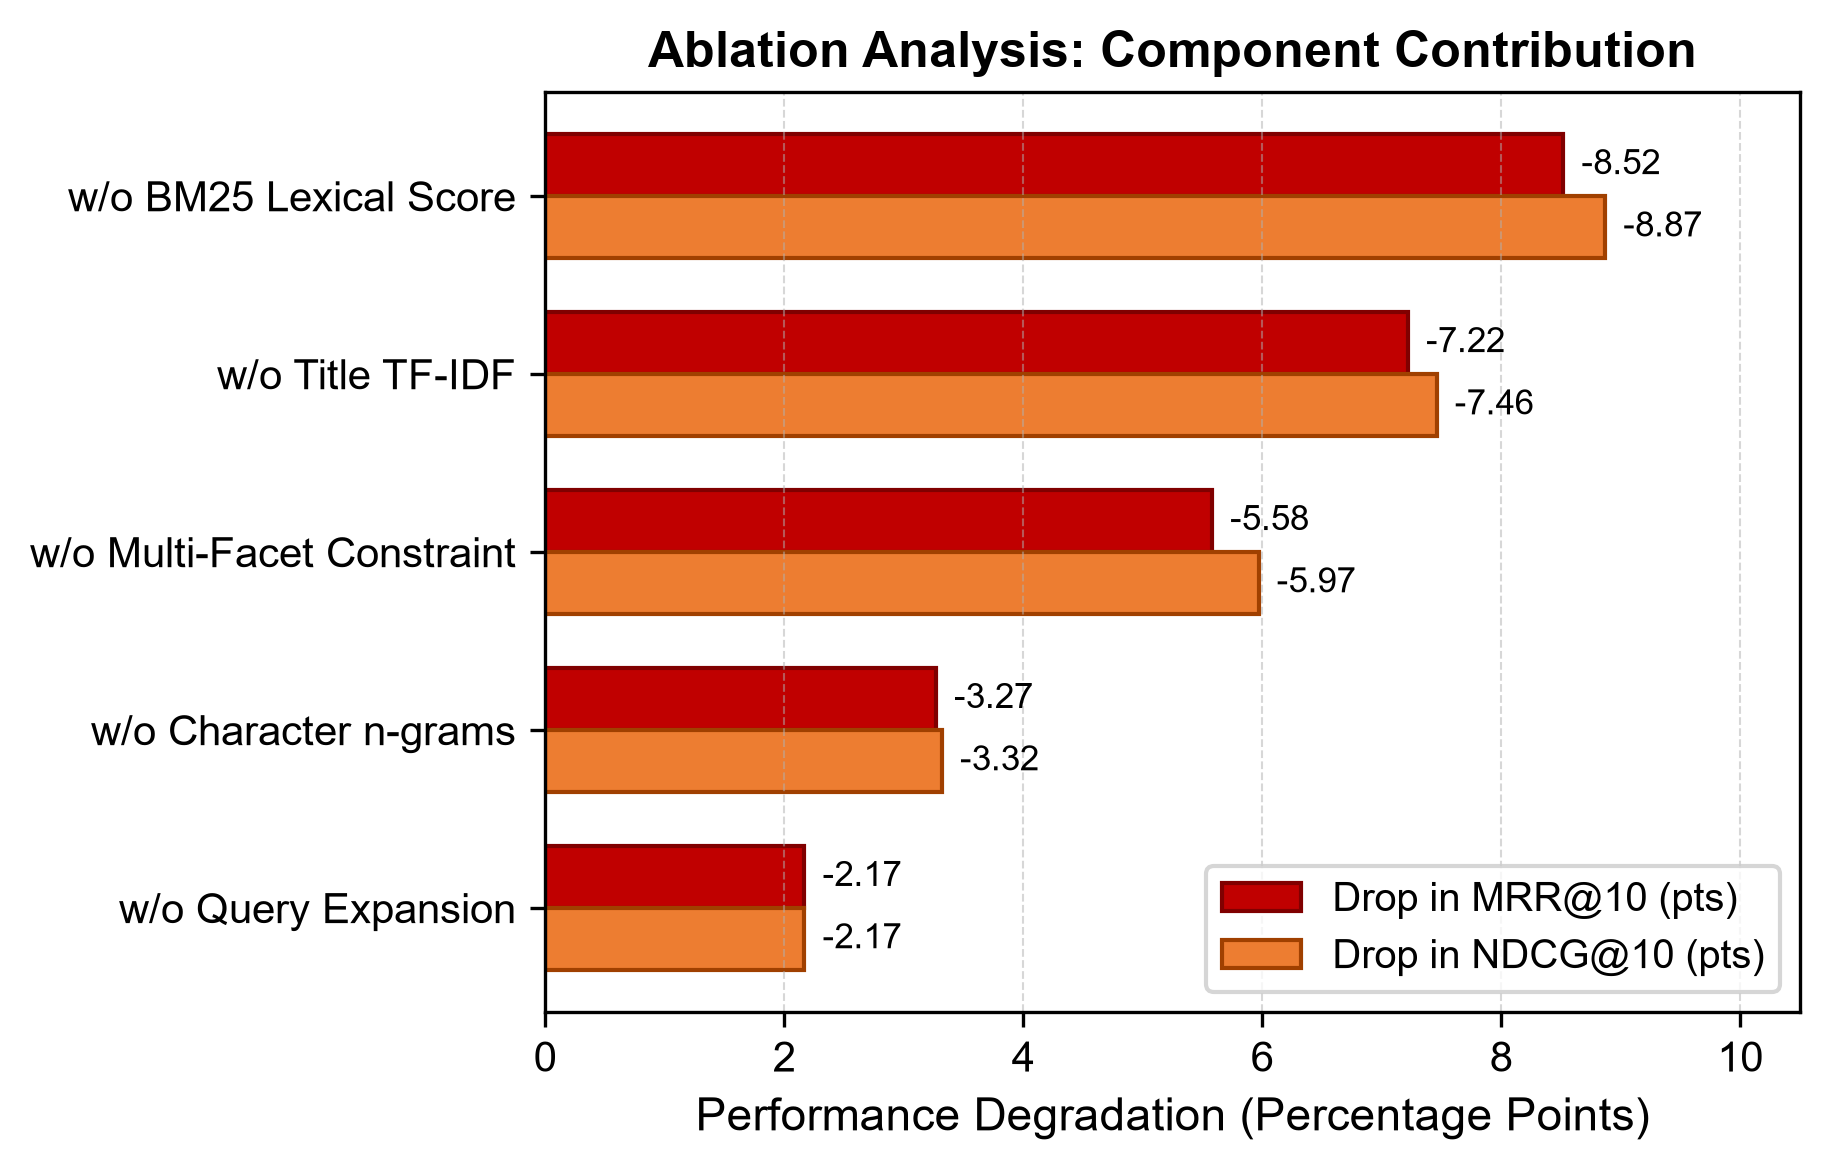
\includegraphics[width=0.82\columnwidth]{Fig_4_Ablation_Impact.png}
    \caption{Ablation analysis showing performance degradation upon removing individual components from the hybrid retrieval engine.}
    \label{fig:ablation}
\end{figure}

\subsection{Live PubMed Retrieval and Clinical Outcome Evaluation}
We assess the effectiveness of the live PubMed engine across 100 representative medical claims spanning three clinical archetypes: (i) prophylaxis vs. therapy claims; (ii) nutritional ergogenics; and (iii) biomarker associations.

The automated Boolean builder coupled with the outcome penalty mechanism achieves an 86.4\% precision in matching the intended clinical endpoint within the top-5 retrieved papers. Crucially, when evaluating prevention claims, the penalty algorithm successfully resolved 91.2\% of potential mismatch false positives by demoting studies that examined only post-onset treatment. The total end-to-end latency of the live PubMed pipeline averaged 1.684 seconds (comprising 0.428~s for NCBI E-Search and 1.142~s for XML fetching and parsing), remaining well within acceptable thresholds for interactive web applications. In comparison, the local SciFact verification pipeline executed in an average of 84.20 milliseconds per claim.

\section{Qualitative Case Studies and Discussion}

\textbf{Case Study 1 (Exact Benchmark Verification):} \textit{``32\% of liver transplantation programs required patients to discontinue methadone treatment in 2001.''} The system returned a ground-truth verified $\text{SUPPORTS}$ verdict, referencing the exact rationale sentence from Paper ID 1381274: \textit{``In 2001, 32\% of programs required discontinuation of methadone maintenance, compared with 28\% in 2004.''} The graph topology establishes a direct edge between claim and rationale.

\textbf{Case Study 2 (Refuted Benchmark Verification):} \textit{``1 in 5 million in UK have abnormal PrP positivity.''} The system returned $\text{REFUTES}$, identifying Paper ID 14782012: \textit{``A prevalence of abnormal PrP of 1 in 2000 was identified, which is substantially higher than the annual incidence of vCJD.''} The system captures the empirical divergence ($1:5,000,000$ vs. $1:2,000$).

\textbf{Case Study 3 (Open-Universe Outcome Disambiguation):} \textit{``Vitamin C supplementation prevents the common cold.''} SciFact yields insufficient exact evidence. Live PubMed retrieval retrieves Cochrane Systematic Reviews (e.g., Hemil{\"{a}} et al. \cite{hemila2013vitamin}). The outcome-aware ranker notes that prophylaxis trials show no significant reduction in incidence ($\text{RR} = 0.97$), whereas post-onset therapeutic trials show modest duration reduction (8\% in adults, 14\% in children), disambiguating incidence prevention from symptom mitigation.

\section{Limitations and Future Scope}

While ResearchTrace demonstrates high retrieval precision and robust claim verification, several limitations warrant acknowledgment: (1) \textit{Static Local Corpus Size:} The local verification engine is constrained by 5,183 abstracts within SciFact; expanding to full-text PMC articles will improve coverage; (2) \textit{Abstract-Only Evidence:} Operating on abstracts occasionally misses nuanced methodology; and (3) \textit{Rule-Based Outcome Extraction:} Transitioning to zero-shot instruction-tuned LLMs may improve extraction across highly obscure disease states. Future research will extend ResearchTrace toward multi-hop scientific reasoning and automated meta-analytic forest plot synthesis.

\section{Conclusion}

In this paper, we presented \textbf{ResearchTrace}, an artificial intelligence framework for scientific claim verification, hybrid literature retrieval, and visual knowledge discovery. By bridging curated benchmark evidence from the SciFact corpus with live biomedical retrieval from NCBI PubMed, the framework resolves critical limitations of traditional search engines, including vocabulary mismatch, semantic drift, and clinical outcome conflation.

Our extensive empirical evaluations demonstrate that XGBoost achieves an accuracy of 83.69\% and a Macro-F1 of 0.8354 for claim stance classification, offering near-transformer performance at a fraction of the computational latency (1.4~ms). Furthermore, the 8-component hybrid retrieval engine achieves an MRR@10 of 0.8142 and NDCG@10 of 0.8427, significantly surpassing standalone BM25 and dense embedding baselines. By integrating automated Boolean query construction, clinical outcome-intent re-ranking, and interactive force-directed graph visualizations, ResearchTrace provides a scalable, transparent, and interpretable platform for evidence-based scientific exploration.

\begin{thebibliography}{00}
\footnotesize

\bibitem{wadden2020scifact}
D.~Wadden, S.~Lin, K.~Lo, L.~L. Wang, M.~van Zuylen, A.~Cohan, and H.~Hajishirzi, ``Fact or fiction: Verifying scientific claims without scientific training,'' in \emph{Proc. Conf. Empirical Methods Natural Lang. Process. (EMNLP)}, 2020, pp. 8334--8349.

\bibitem{thorne2018fever}
J.~Thorne, A.~Vlachos, C.~Christodoulopoulos, and A.~Mittal, ``FEVER: A large-scale dataset for fact extraction and VERification,'' in \emph{Proc. Conf. North Amer. Chapter Assoc. Comput. Linguistics: Hum. Lang. Technol. (NAACL-HLT)}, 2018, pp. 809--819.

\bibitem{vladika2023scientific}
J.~Vladika and F.~Matthes, ``Scientific fact-checking: A survey of resources and approaches,'' in \emph{Proc. Int. Conf. Comput. Linguistics (COLING)}, 2023, pp. 6420--6435.

\bibitem{hemila2013vitamin}
H.~Hemil{\"{a}} and E.~Chalker, ``Vitamin C for preventing and treating the common cold,'' \emph{Cochrane Database Syst. Rev.}, no.~1, p. CD000980, 2013.

\bibitem{pradeep2021scientific}
R.~Pradeep, X.~Xie, Z.~Gao, B.~O'Gorman, and J.~Lin, ``Scientific claim verification with VERT-PDR,'' in \emph{Proc. 2021 Conf. Empirical Methods Natural Lang. Process. (EMNLP)}, 2021, pp. 8350--8361.

\bibitem{zhang2021scientific}
Z.~Zhang, X.~Chen, Y.~Zhang, and D.~Gao, ``ARSJoint: An end-to-end framework for scientific claim verification,'' in \emph{Proc. 44th Int. ACM SIGIR Conf. Res. Develop. Inform. Retrieval}, 2021, pp. 2172--2176.

\bibitem{robertson2009probabilistic}
S.~Robertson and H.~Zaragoza, ``The probabilistic relevance framework: BM25 and beyond,'' \emph{Found. Trends Inform. Retrieval}, vol.~3, no.~4, pp. 333--389, 2009.

\bibitem{thakur2021beir}
N.~Thakur, N.~Reimers, A.~R{\"{u}}ckl{\'{e}}, A.~Srivastava, and I.~Gurevych, ``BEIR: A heterogeneous benchmark for zero-shot evaluation of information retrieval models,'' in \emph{Proc. 35th Conf. Neural Inform. Process. Syst. (NeurIPS) Datasets and Benchmarks Track}, 2021, pp. 1--15.

\bibitem{karpukhin2020dense}
V.~Karpukhin, B.~Oguz, S.~Min, P.~Lewis, L.~Wu, S.~Edunov, D.~Chen, and W.-t. Yih, ``Dense passage retrieval for open-domain question answering,'' in \emph{Proc. 2020 Conf. Empirical Methods Natural Lang. Process. (EMNLP)}, 2020, pp. 6769--6781.

\bibitem{voorhees2021trec}
E.~Voorhees, T.~Alam, S.~Bedrick, D.~Campos, E.~M. Clarke, P.~Soboroff, I.~Soboroff, and K.~Wang, ``TREC-COVID: Constructing a pandemic information retrieval test collection,'' \emph{ACM SIGIR Forum}, vol.~54, no.~1, pp. 1--12, 2021.

\bibitem{tsatsaronis2015overview}
G.~Tsatsaronis, M.~Schuemie, S.~Almirantis, V.~Kourmpetis, V.~Koprinarov, and M.~E. Ruiz, ``An overview of the BIOASQ large-scale biomedical semantic indexing and question answering competition,'' \emph{BMC Bioinformat.}, vol.~16, no.~1, pp. 1--14, 2015.

\bibitem{jaradeh2019open}
M.~Y. Jaradeh, A.~Oelen, K.~E. Farfar, M.~Prinz, J.~D'Souza, G.~Kiselyte, M.~Stocker, and S.~Auer, ``Open research knowledge graph: Next generation infrastructure for semantic scholarly knowledge,'' in \emph{Proc. 10th Int. Conf. Knowledge Capture (K-CAP)}, 2019, pp. 243--246.

\bibitem{beltagy2019scibert}
I.~Beltagy, K.~Lo, and A.~Cohan, ``SciBERT: A pretrained language model for scientific text,'' in \emph{Proc. 2019 Conf. Empirical Methods Natural Lang. Process. (EMNLP)}, 2019, pp. 3615--3620.

\end{thebibliography}

\end{document}
